%Author of the LaTeX-class is Lennart Franked
%Main author of the contents in the thesis template is Stefan Forsström at Mid Sweden University

%When writing your thesis in Swedish, only change in the documentclass from English to Swedish. All
%section headings that have a translate will automatically be changed to the swedish translation.

%\documentclass[english]{miunthesis}
\documentclass[english]{miunthesis}
\usepackage{csquotes}
\usepackage{booktabs}
\usepackage{float}
\usepackage{newfloat}
\usepackage[]{appendix}

\addbibresource{literature.bib}

\title{Title}
\subtitle{Subtitle}
\author{Author}

\projecttype{course name/specialisation from the course syllabus}

\fieldofstudy{Computer Science}
\coursecredits{30 hp}

\supervisor{John Doe}
\examiner{Nomen Nescio}

\coursecode{DTXXX} % Optional
\registrationnr{DT-085H-WER} % Optional

\studyprogramme{Master programme} % Optional

\begin{document}
  \maketitle
  \pagenumbering{roman}
  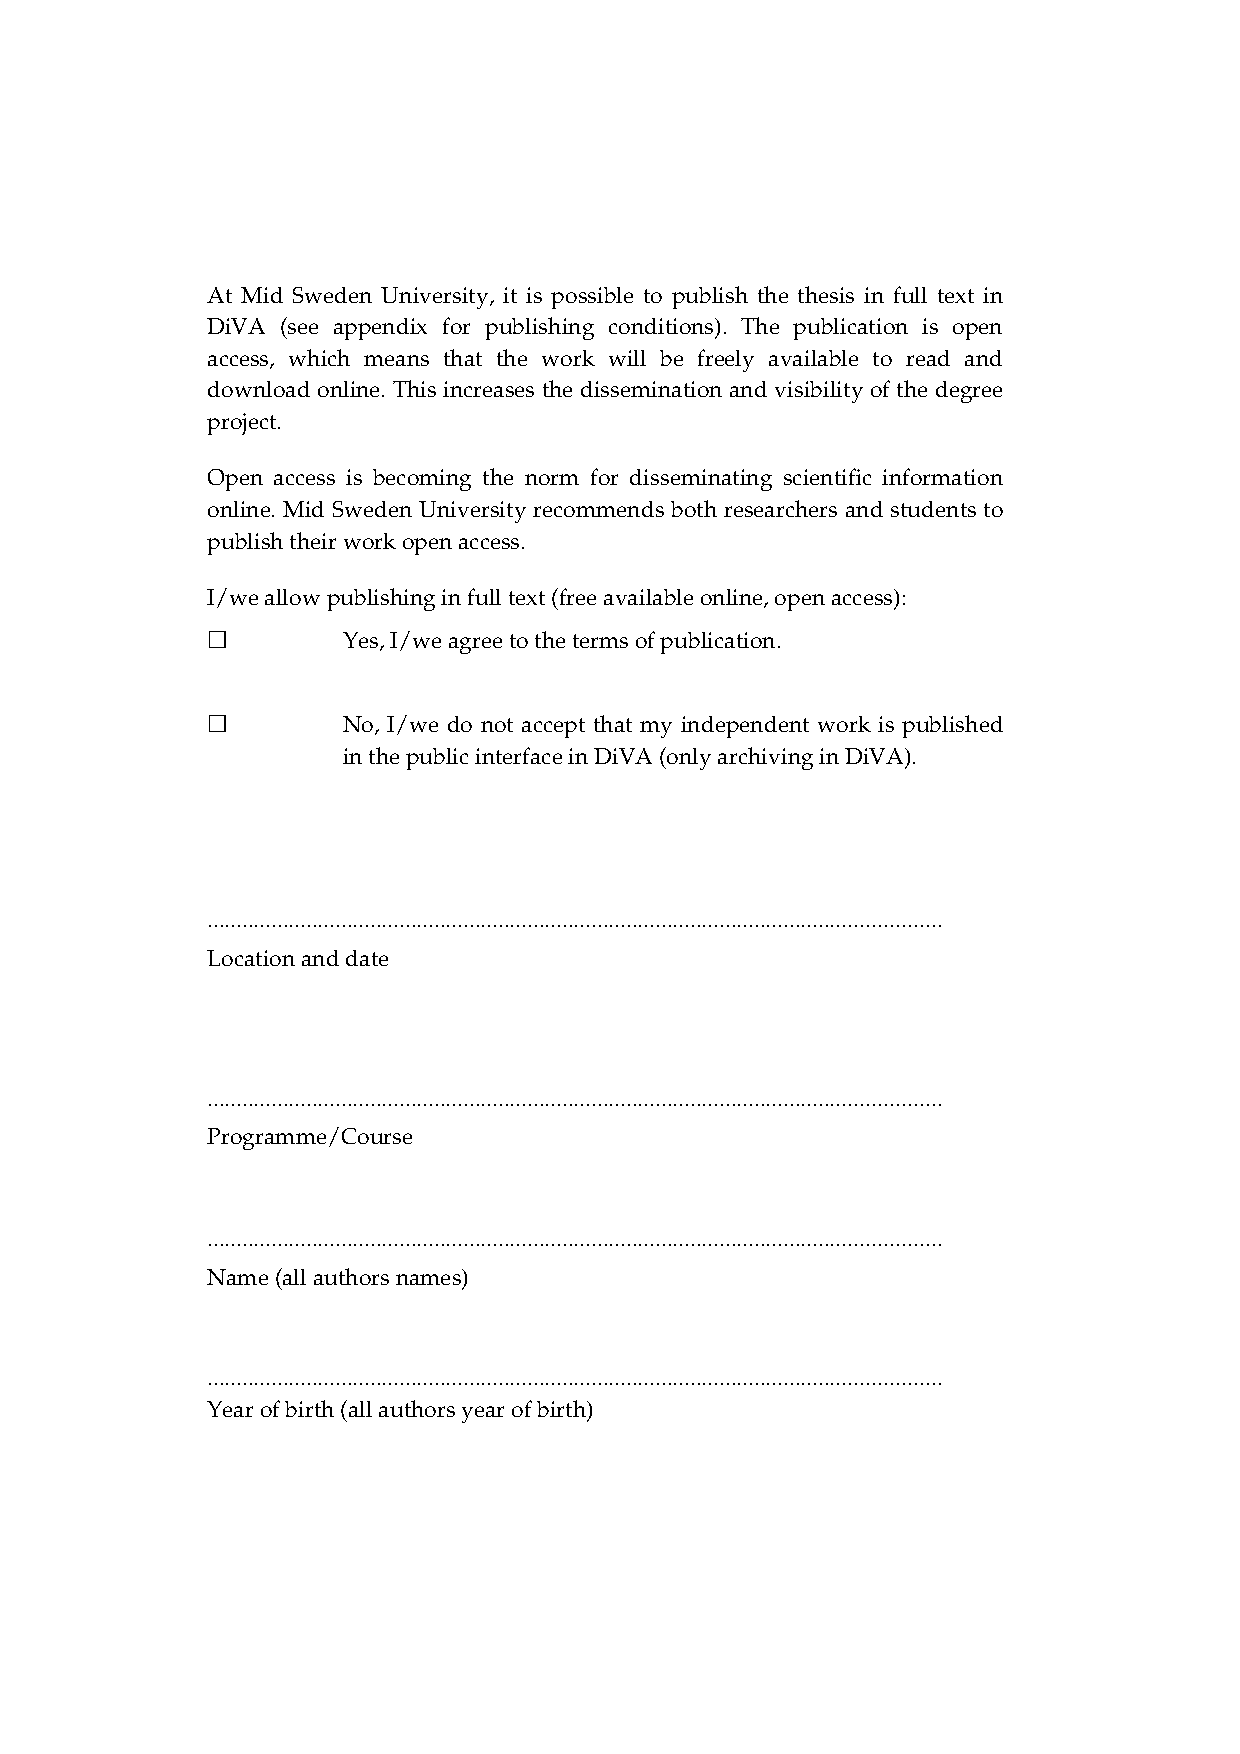
\includepdf[pages=1]{Diva_publish.pdf}
  \newpage
  \printabstract
  
  \section*{\translate{Acknowledgements}}\label{sec:acknowledgements}
\phantomsection
\addcontentsline{toc}{section}{\translate{Acknowledgements}} 
Acknowledgements are not mandatory but can be applied if you as the writer wish to provide general
information about your exam work or project work, educational programme, institution, business,
tutors and personal comments, i.e.\ thanks to any persons that may have helped you. Acknowledgements
are to be placed on a separate page.

  \newpage
  
  \tableofcontents
  \newpage

  \phantomsection
  \listoffigures
  \addcontentsline{toc}{section}{\translate{List of Figures}}
  \newpage

  \phantomsection
  \listoftables
  \addcontentsline{toc}{section}{\translate{List of Tables}}
  \newpage

  \phantomsection
  \listofalgorithms
  \addcontentsline{toc}{section}{\translate{List of Algorithms}}
  \newpage

  \section*{Terminology}\label{sec:terminology}
\phantomsection
\addcontentsline{toc}{section}{Terminology}
\begin{table}[ht!]
  \begin{tabular}{l l}
DL & Description Logic\\
GDPR & General Data Protection Regulation\\
ICT & Information and Communication Technologies\\
ILO & Intended Learning Outcome\\
MCQ & Multiple Choice Questions\\
SBA & Single Best Answer\\
\end{tabular}
\end{table}

  \newpage
  \pagenumbering{arabic}
  \section{\translate{Introduction}}\label{sec:intro}
During your previous education, you have probably come across relatively well
defined problem types as formulated by teachers, textbooks and teaching aids.
During project courses and exam work you are required to do a great deal of the
thinking by yourself in order to define and clarify the direction of the
assignment. This analysis should be presented in the report's introductory
chapter. By describing the problem or problem area chosen for study and the
reasons behind this choice, it should then be possible to write a general
introduction to the report. The introductory chapter relates to the content in
the project plan that will be presented some weeks after the diploma work has
started. The project plan should also contain a time plan for the work. The
project plan can also mention some of the intended sources to be read and
subsequently referred to in chapter 2, and also to contain some thoughts about
the method (see chapter 3) chosen in order to approach the problem. The
introduction making up chapter 1, may also contain sub-headings underneath. Try
to get to the point as soon as possible. In order to retain the reader’s
interest information concerning your work must be given within the first few
sentences. People only requiring a quick insight into the work will often only
read the report's summary, introduction and conclusions, since these sections
are usually written without the inclusion of highly technical and mathematical
details.

\subsection{\translate{Background and problem motivation}}\label{subsec:background}
\noindent 
In this sub-chapter you should try to quickly engage the readers' interest in
the problem area you have chosen to examine. Demonstrate that you are not only
familiar with any minor technical problems, but also have an understanding of
the context in which your problem emerges, that you can also describe it from a
non-technical perspective, and that you are aware of the practical benefits of
the technology you are examining or have knowledge of areas that your study
relates to. It is common that the first sentence contains an insightful
formulation or historical retrospective. Obviously it is not possible to be
absolutely certain with regards to the future, but you should express your
hypothesis in a balanced and objective manner in order to appear credible.

Examples: ``Humankind during historical times has\dots. The use of internet and
cellular telephony has grown since\dots. The next stage in the development is
expected to become\dots. This can lead to problems with… This study investigates if
the problem can be solved with the aid of\dots. This technology can become
especially interesting if in some years many more people\dots, and there is a
growing demand on the market after\dots''.
A technical report that is carried out on behalf of a company could start with:
“Within the organization there is an increased need for\dots and at the same time

\subsection{\translate{Overall aim}}\label{subsec:aim}
\noindent
The project's aim is an insightful description of the direction in which you
want to work, your hopes with regards to the possible outcomes of the project,
and of the projects' purpose. The hypothesis does not need to be clearly defined
or concrete. It can be an objective which may or may not be resolved or achieved
with any degree of certainty. It can be a problem formula of a high level, which
cannot be answered by the study's diagrams, tables and other objective results,
but which can be discussed in the report's concluding chapter. Examples: ``the
project's overall aim is to gain new knowledge within the organization
about\dots''.
``The project's aim is to identify the general valid principles for the
connection between parameter X and Y for everybody\dots''. ``The project's aim is to
find new technical solutions to problems in the following area:\dots.'' ``The
project's aim is to compare technology A with technology B as a solution to the
needs of C.'' ``The project aims to present a decision-making basis for\dots''
``The project aims to investigate whether or not it is realistic to expect that
technology A could be used for purpose B in the future.''

\subsection{\translate{Scope}}\label{subsec:scope}
\noindent
Examples: ``The study has its focus on\dots. In the survey, the effect of parameter Z
is ignored, because…. The survey is distinguished by the evaluation of cases F1
and F2\dots. The survey's conclusions should however be generally valid for
every\dots.''

\subsection{\translate{Concrete and verifiable goals}}\label{subsec:goals}
\noindent
The problem- or objective statement is a verification of the proposed formula
you will use to reach your objective. The questions that are specified should be
answered in the report's results, and in its conclusion. The problem statement
should be so clearly defined that deciding whether or not the problem has been
resolved should be an easy process. This sub-chapter is usually written after
the implementation of the theoretical
study in chapter 2, and should be revised at regular intervals throughout the
duration of the project. The problem statement might in some cases require to be
placed after the theoretical study. This way of writing a study may be used if
it seems to be difficult for the reader to understand the concepts used. The
disadvantage of such a layout is that the reader might lose interest in the
subject before the core points have been stated. Examples of problem statements
useful in a scientific report are ``the survey has
an objective to respond to the following questions: P1: What importance has
technology A compared with technology B for the performance measure Y at
different values on parameter X, for cases F1 and F2? P2: Which profit gives…
For mathematical definitions of X and Y, see the model in chapter 3.'' It is then
in chapter 3 that the objective numerical results will be specified, i.e.\ what
will exist on the x - and y-axis in the diagram you intend to take further.
Examples of objectives for a technical report: ``the survey's objective is to
suggest a solution to the following technical problems:\dots the survey has
further objectives to verify that the solution proposal provides useable
criteria and to evaluate the proposal with respect to performance measure Y.''
All technical details are reserved for the structure chapter's technical
requirement specifications.

\subsection{\translate{Outline}}\label{subsec:outline}
\noindent
Briefly describe the report's outline. ``Chapter 2 describes\dots''

\subsection{\translate{Contributions}}\label{subsec:contributions}
\noindent 
Describe which parts of the work that you have conducted yourself, and which
parts that you had help with i.e.\ carried out by colleagues. If the work is
carried out in a group the report should then explain how the tasks were divided
between authors. All co-authors should be credited in the work as a whole.

  \section{Theory}\label{sec:theory}


  \section{\translate{Methodology}}\label{sec:method}
Summarize and introduce the methodology chapter. The method section is the point
at which your chosen method and intended procedure are presented. This section
should contain information for the reader to interpret your results and repeat
your work, i.e.\ in order to check the results. Here, the tools, assumptions,
mathematical models, performance measures and assessment criteria are presented.

\subsection{\translate{Scientific method description}}\label{subsec:scientificmethod}
Explain your scientific method. Quantitative method? Design science? Engineering research? etc. 

Explain how you will attack and work with each of the scientific/knowledge
goals/research questions. One paragraph per scientific goal/question is often
enough.

\subsection{\translate{Project method description}}\label{subsec:projectmethod}

Explain your project method. Split the work into a number of achievable milestones/phases. Many
theses work in computer engineering are typically split into the following parts: 
\emph{Theory} (in which you will gain more knowledge to be able to solve the problem),
\emph{Pre-study} (where you will further refine your requirements, approach, design, etc.),
\emph{Implementation} (where you will build some artifact), Measure (in which you will perform
measurements on your artifact), and \emph{Evaluation} (where you will analyze and evaluate your
results and measurements).  

Explain how you will work and do within each of these milestones/phases. Justify
your choice of methodology/model. What metrics will you use to evaluate your work? Comment on the
method's possible weaknesses and problems that may arise during actual implementation. A flowchart
can help in visualizing the work. One paragraph per milestone/phase is often enough to write.

\subsection{\translate{Project evaluation method}}\label{subsec:evalmethod}
How will you look back upon your whole thesis work in the end and evaluate if it
was a success? Focus on your whole thesis project process and remember that this
is different from your measurements/evaluation of your implementation.

  \section{\translate{Pre study}/\translate{Approach}}\label{sec:prestudy} 

Choose only one of the headlines. This chapter will be substantially different depending on your
thesis topic, direction, and scientific level. But in this chapter, you will present the different
options you have faced and made your choice between, or you will explain the pre-study that has led
up to your design, implementation, and your analysis of different requirement.        

\subsection{\translate{Requirements capturing}/\translate{Approach alternatives}}\label{subsec:solutionalt}
Explain the requirement capturing and the identified requirements, or the different approach alternatives.

\subsubsection{Alternative X/Approach X}\label{subsubsec:altx}
Present and summarize the potential approaches or requirements that you have considered. Make them
even in length and style, to be of equal in importance. Continue the list with all
alternatives/requirement, one heading for each.

\subsubsection{Another requirement/alternative}
Another requirement or potential approach.

\subsubsection{Etc.\ until all has been covered}
Another, etc.

\subsection{\translate{Requirement analysis}/\translate{Comparison of
    approaches}}\label{subsec:compareapproach}
Analyze the identified requirements, compare different approaches to another, benefits, drawbacks?
Pros vs cons? A table for clear comparison can be used, for example a Pugh matrix.

\subsection{\translate{Proposed approach}/\translate{Chosen approach}}\label{subsec:chosenapproach}
Present your proposed or chosen approach. It is very important to motivate why this was chosen over
the others. Connect back to your overall aim and problem statement, to ensure that the chosen
approach actually can answer your scientific goals/research questions.


  \section{\translate{Implementation}/\translate{Design}}\label{sec:implementation} 
Choose only one of the headlines. In this chapter you will explain all the technical details of your
work. Start this chapter with an overview of your work and an overview block figure with the
protocols, algorithms, and technologies written out. Basically, as form of UML component diagram.
You can also use storyboards, mock-up designs, state diagrams to show the overall structure. See
Figure 1 for an example. All figures must be references from the text. 
\cref{fig:overview}. All figures must be references from the text.

\begin{figure}
  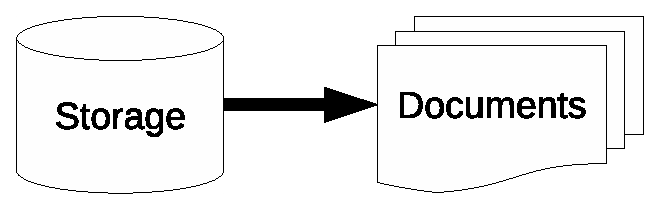
\includegraphics[width=5cm]{Figures/Latex_figure1.eps}
  \caption{System overview}\label{fig:overview}
\end{figure}

\subsection{First part of the overview figure}\label{subsec:overview1}
Use a top-down approach, divide and conquer, split the figure into relevant pieces. Explain each
piece in detail, use titles that can be found in the overview figure. Use flow charts, UML diagram,
pseudocode etc.\ but no real code. Refer to the appendix for the actual source code.

\subsection{Another part of the overview figure}\label{subsec:overview2}
Another piece of the solution.

\subsection{Etc.\ until all parts are covered from the overview figure}
Another piece of the solution. Etc.\

\subsection{\translate{Measurement}/
            \translate{Evaluation setup}}\label{subsec:eval_setup} 

Remember to explain how you will measure/evaluate your implementation and how your test bench has
been built/setup/implemented.

  \section{\translate{Results}}\label{sec:results}
Summarize and introduce your results

\subsection{\translate{Resulting application}/\translate{Resulting system}}\label{subsec:resultapp}
Present your resulting work. Screenshots, features, etc.

\subsection{\translate{Measurement results}}\label{subsec:measurementresults}
Present your measurements. How well does it perform? Present the results objectively, with as little
bias as possible. Use tables, graphs, etc.  You can find an example table below. See Table 1.

\begin{table}
  \caption{Measured times for the model.}
  \begin{tabular}{c c c c c}
              & Shortest (ms) & Longest (ms) & Average (ms) & Stdev (ms)\\
    \toprule
    Model one & 10 & 30 & 20 & 5 \\
    \midrule 
    Model two & 20 & 40 & 35 & 3 \\
    \bottomrule
  \end{tabular}
\end{table}

Here is an example of a line graph. See~\cref{fig:line}.
\begin{figure}
  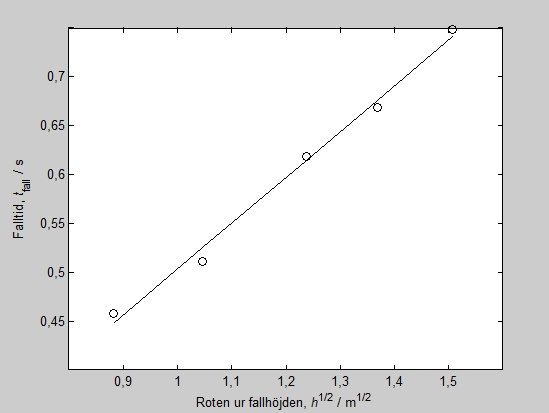
\includegraphics[width=5cm]{Figures/graph1.png}
  \caption{Line graph example.}\label{fig:line}
\end{figure}

Here is an example of a bar chart with standard deviation whiskers. See~\cref{fig:bar}.
\begin{figure}
  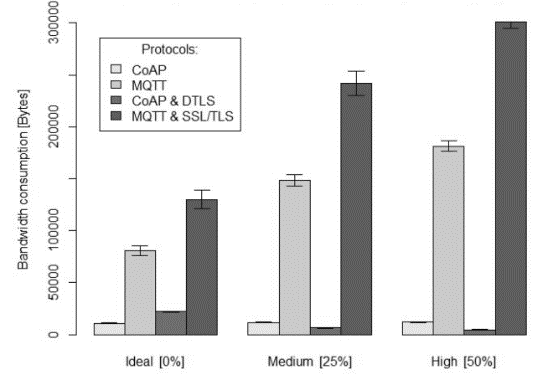
\includegraphics[width=5cm]{Figures/graph2.png}
  \caption{Bar chart example.}\label{fig:line}
\end{figure}

Here is an example boxplot. See~\cref{fig:boxplot}

\begin{figure}
  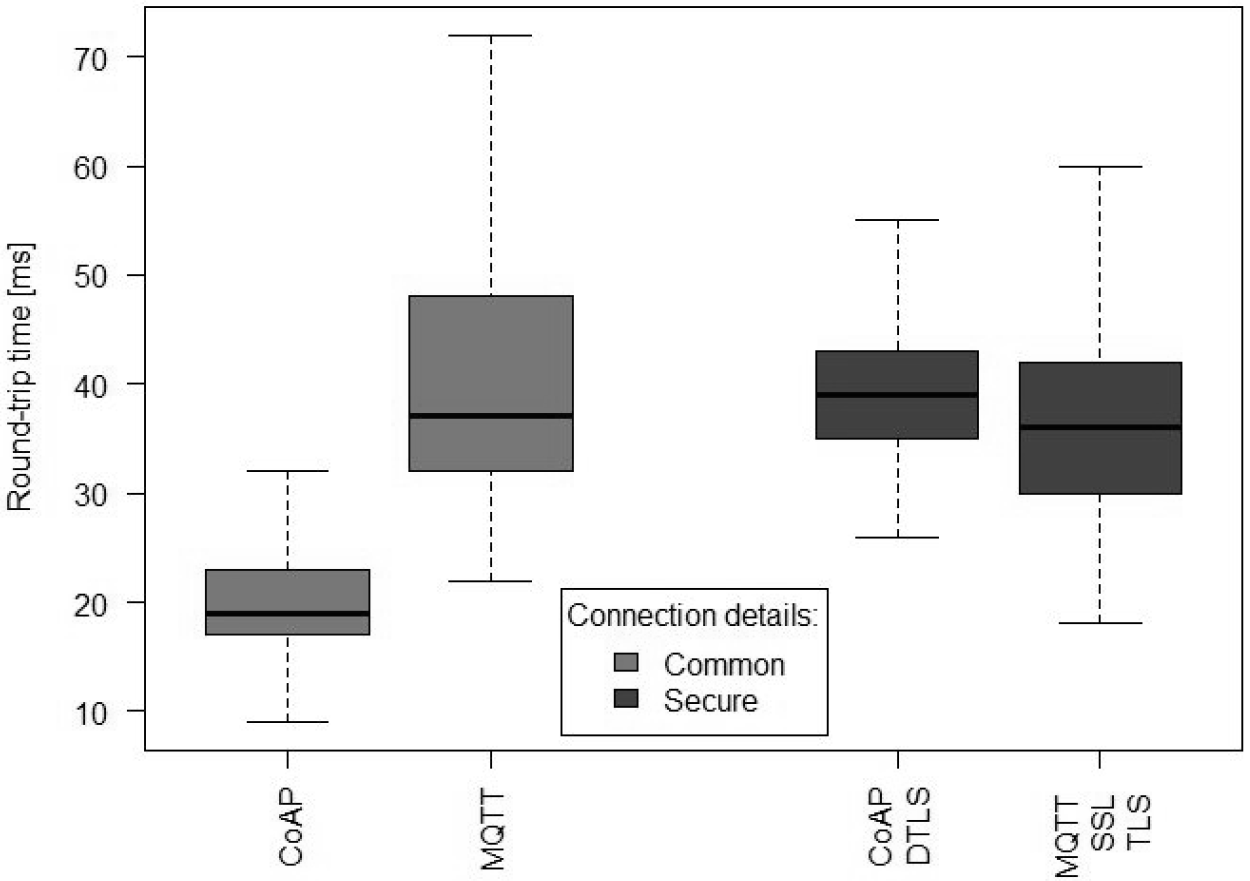
\includegraphics[width=5cm]{Figures/graph3.png}
  \caption{Boxplot example.}\label{fig:line}
\end{figure}

Here is an example equation. See~\cref{eqn:exampleeqn}

\begin{equation}
  P_{i,j} = C\frac{P_iG_{i,j}}{d^a_{i,j}}
\end{equation}

  \section{\translate{Discussion}}\label{sec:discussion}
Summarize and introduce what you will discuss and analyze.

\subsection{\translate{Analysis and discussion of results}}\label{subsec:discussion_analysis}
Make a deep analysis and discussion of your resulting application, measurements,
evaluation, etc. Here it is ok to be more subjective/biased.

\subsection{\translate{Project method discussion}}\label{subsec:project_method_discussion}
Make a deep analysis and discussion of your chosen method, chosen approach,
chosen metrics, etc. Answer all of your project phases/milestones. Have they
been met?

\subsection{\translate{Scientific discussion}}\label{subsec:scientific_discussion}
Make a deep discussion of the gained scientific knowledge and your scientific
method. What can be learnt? Is this knowledge general or specific, etc. Make a
discussion by looking back at the related works and put your work into
perspective. Remember to discuss and show insights into the scientific
possibilities of this work and its limitations

\subsection{\translate{Ethical and societal discussion}}\label{subsec:ethical_discussions}
You will need to include a discussion on ethics, societal impact, and
considerations. Use the human perspective, how will we be effected by this work,
was people involved in the process, privacy? Remember to discuss and show
insights into this projects role in society and our responsibilities for how it
is used.

  \section{\translate{Conclusion}}\label{sec:conclusions}

Summarize your outcome. Answer all of your scientific/knowledge goals/research
questions. Have they been met?

Answer your problem statement.

Make clear conclusions regarding your goals, research questions and problem
statement. Include your scientific contribution and impact.

\subsection{\translate{Future Work}}\label{subsec:future_work}
You should also explain potential future work based on your work.

\subsection{Example of a future work}\label{subsec:example_future_work}
Remember to not just point out potential future work, also explain how you would
approach this particular future work if you had the opportunity to do so.



  \addcontentsline{toc}{section}{\translate{References}}
  \printbibliography{}
  \newpage\clearpage
  \pagestyle{fancy}
  \setcounter{page}{1}
  \appendix
  \noappendicestocpagenum
  \section{\translate{Appendice} A}\label{sec:appA}
\end{document}
